\section*{Languages and Frameworks}
In order to test our system, we need to use a tool to create a \textit{virtual network} inside our machine; we used \texttt{mininet}, 
exploiting the \texttt{python2} APIs. To simulate input from an external application we also used a python2 library, called \texttt{requests},
which is able to act like an HTTP client.

\section{Scenario}
We want to simumlate a tipical data center scenario with a single LAN, implemented in a \textit{Spine-Leaf} topology. This configuration
is widely used thanks to it's easy scalability and sufficent redundancy.
\begin{figure}[h]
    \caption{example of \textit{spine-leaf} topology}
    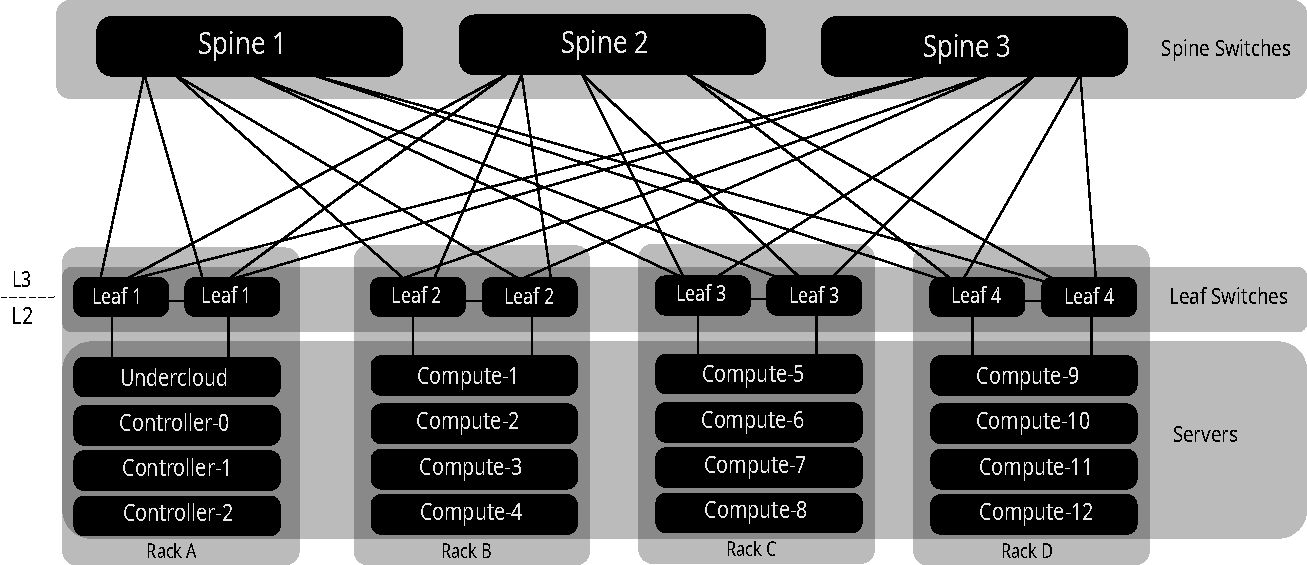
\includegraphics[width=0.90\textwidth]{img/spine_leaf.pdf}
\end{figure}

Using \texttt{mininet}, we can also simulate an episode of link failure, in order to test the system behaviour in this specific case. The system is able to
recompute a functional path between two host and use it to forward packets.
